\documentclass[twoside]{book}

% Packages required by doxygen
\usepackage{fixltx2e}
\usepackage{calc}
\usepackage{doxygen}
\usepackage[export]{adjustbox} % also loads graphicx
\usepackage{graphicx}
\usepackage[utf8]{inputenc}
\usepackage{makeidx}
\usepackage{multicol}
\usepackage{multirow}
\PassOptionsToPackage{warn}{textcomp}
\usepackage{textcomp}
\usepackage[nointegrals]{wasysym}
\usepackage[table]{xcolor}

% Font selection
\usepackage[T1]{fontenc}
\usepackage[scaled=.90]{helvet}
\usepackage{courier}
\usepackage{amssymb}
\usepackage{sectsty}
\renewcommand{\familydefault}{\sfdefault}
\allsectionsfont{%
  \fontseries{bc}\selectfont%
  \color{darkgray}%
}
\renewcommand{\DoxyLabelFont}{%
  \fontseries{bc}\selectfont%
  \color{darkgray}%
}
\newcommand{\+}{\discretionary{\mbox{\scriptsize$\hookleftarrow$}}{}{}}

% Page & text layout
\usepackage{geometry}
\geometry{%
  a4paper,%
  top=2.5cm,%
  bottom=2.5cm,%
  left=2.5cm,%
  right=2.5cm%
}
\tolerance=750
\hfuzz=15pt
\hbadness=750
\setlength{\emergencystretch}{15pt}
\setlength{\parindent}{0cm}
\setlength{\parskip}{0.2cm}
\makeatletter
\renewcommand{\paragraph}{%
  \@startsection{paragraph}{4}{0ex}{-1.0ex}{1.0ex}{%
    \normalfont\normalsize\bfseries\SS@parafont%
  }%
}
\renewcommand{\subparagraph}{%
  \@startsection{subparagraph}{5}{0ex}{-1.0ex}{1.0ex}{%
    \normalfont\normalsize\bfseries\SS@subparafont%
  }%
}
\makeatother

% Headers & footers
\usepackage{fancyhdr}
\pagestyle{fancyplain}
\fancyhead[LE]{\fancyplain{}{\bfseries\thepage}}
\fancyhead[CE]{\fancyplain{}{}}
\fancyhead[RE]{\fancyplain{}{\bfseries\leftmark}}
\fancyhead[LO]{\fancyplain{}{\bfseries\rightmark}}
\fancyhead[CO]{\fancyplain{}{}}
\fancyhead[RO]{\fancyplain{}{\bfseries\thepage}}
\fancyfoot[LE]{\fancyplain{}{}}
\fancyfoot[CE]{\fancyplain{}{}}
\fancyfoot[RE]{\fancyplain{}{\bfseries\scriptsize Generated on Sun Nov 15 2015 22\+:09\+:00 for Gym\+Pesicka\+V00807592 by Doxygen }}
\fancyfoot[LO]{\fancyplain{}{\bfseries\scriptsize Generated on Sun Nov 15 2015 22\+:09\+:00 for Gym\+Pesicka\+V00807592 by Doxygen }}
\fancyfoot[CO]{\fancyplain{}{}}
\fancyfoot[RO]{\fancyplain{}{}}
\renewcommand{\footrulewidth}{0.4pt}
\renewcommand{\chaptermark}[1]{%
  \markboth{#1}{}%
}
\renewcommand{\sectionmark}[1]{%
  \markright{\thesection\ #1}%
}

% Indices & bibliography
\usepackage{natbib}
\usepackage[titles]{tocloft}
\setcounter{tocdepth}{3}
\setcounter{secnumdepth}{5}
\makeindex

% Hyperlinks (required, but should be loaded last)
\usepackage{ifpdf}
\ifpdf
  \usepackage[pdftex,pagebackref=true]{hyperref}
\else
  \usepackage[ps2pdf,pagebackref=true]{hyperref}
\fi
\hypersetup{%
  colorlinks=true,%
  linkcolor=blue,%
  citecolor=blue,%
  unicode%
}

% Custom commands
\newcommand{\clearemptydoublepage}{%
  \newpage{\pagestyle{empty}\cleardoublepage}%
}


%===== C O N T E N T S =====

\begin{document}

% Titlepage & ToC
\hypersetup{pageanchor=false,
             bookmarks=true,
             bookmarksnumbered=true,
             pdfencoding=unicode
            }
\pagenumbering{roman}
\begin{titlepage}
\vspace*{7cm}
\begin{center}%
{\Large Gym\+Pesicka\+V00807592 }\\
\vspace*{1cm}
{\large Generated by Doxygen 1.8.10}\\
\vspace*{0.5cm}
{\small Sun Nov 15 2015 22:09:00}\\
\end{center}
\end{titlepage}
\clearemptydoublepage
\tableofcontents
\clearemptydoublepage
\pagenumbering{arabic}
\hypersetup{pageanchor=true}

%--- Begin generated contents ---
\chapter{Hierarchical Index}
\section{Class Hierarchy}
This inheritance list is sorted roughly, but not completely, alphabetically\+:\begin{DoxyCompactList}
\item \contentsline{section}{Exercise}{\pageref{class_exercise}}{}
\begin{DoxyCompactList}
\item \contentsline{section}{Exercise\+Bike}{\pageref{class_exercise_bike}}{}
\item \contentsline{section}{the\+Elliptical}{\pageref{classthe_elliptical}}{}
\item \contentsline{section}{the\+Treadmill}{\pageref{classthe_treadmill}}{}
\item \contentsline{section}{Weight\+Room}{\pageref{class_weight_room}}{}
\end{DoxyCompactList}
\item \contentsline{section}{Factory}{\pageref{class_factory}}{}
\end{DoxyCompactList}

\chapter{Class Index}
\section{Class List}
Here are the classes, structs, unions and interfaces with brief descriptions\+:\begin{DoxyCompactList}
\item\contentsline{section}{\hyperlink{class_exercise}{Exercise} }{\pageref{class_exercise}}{}
\item\contentsline{section}{\hyperlink{class_exercise_bike}{Exercise\+Bike} }{\pageref{class_exercise_bike}}{}
\item\contentsline{section}{\hyperlink{class_factory}{Factory} }{\pageref{class_factory}}{}
\item\contentsline{section}{\hyperlink{classthe_elliptical}{the\+Elliptical} }{\pageref{classthe_elliptical}}{}
\item\contentsline{section}{\hyperlink{classthe_treadmill}{the\+Treadmill} }{\pageref{classthe_treadmill}}{}
\item\contentsline{section}{\hyperlink{class_weight_room}{Weight\+Room} }{\pageref{class_weight_room}}{}
\end{DoxyCompactList}

\chapter{Class Documentation}
\hypertarget{class_exercise}{}\section{Exercise Class Reference}
\label{class_exercise}\index{Exercise@{Exercise}}
Inheritance diagram for Exercise\+:\begin{figure}[H]
\begin{center}
\leavevmode
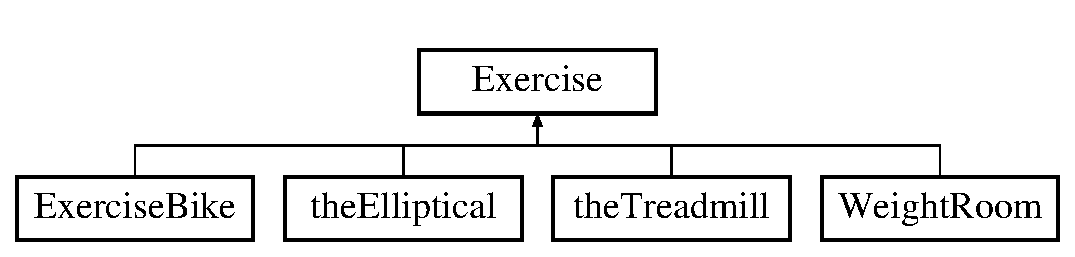
\includegraphics[height=2.000000cm]{class_exercise}
\end{center}
\end{figure}
\subsection*{Public Member Functions}
\begin{DoxyCompactItemize}
\item 
virtual \hyperlink{class_exercise}{Exercise} $\ast$ \hyperlink{class_exercise_ae8dd16c306375ec553ab046e26bea59a}{clone} ()=0
\item 
\hypertarget{class_exercise_a580f318e6ceb6f3d0d2b22c420abefff}{}virtual void {\bfseries work\+\_\+out} ()=0\label{class_exercise_a580f318e6ceb6f3d0d2b22c420abefff}

\end{DoxyCompactItemize}


\subsection{Member Function Documentation}
\hypertarget{class_exercise_ae8dd16c306375ec553ab046e26bea59a}{}\index{Exercise@{Exercise}!clone@{clone}}
\index{clone@{clone}!Exercise@{Exercise}}
\subsubsection[{clone()=0}]{\setlength{\rightskip}{0pt plus 5cm}virtual {\bf Exercise}$\ast$ Exercise\+::clone (
\begin{DoxyParamCaption}
{}
\end{DoxyParamCaption}
)\hspace{0.3cm}{\ttfamily [pure virtual]}}\label{class_exercise_ae8dd16c306375ec553ab046e26bea59a}
string Exercise\+Name; 

Implemented in \hyperlink{class_weight_room_adc9336a7d4d0f826d8e17e3ac2a0b936}{Weight\+Room}, \hyperlink{class_exercise_bike_a399ba0e490a455147245e79ca814be24}{Exercise\+Bike}, \hyperlink{classthe_treadmill_af116aacb6c62a04edd1029a6049c1461}{the\+Treadmill}, and \hyperlink{classthe_elliptical_a650c1be9061ad3c25eda5017d50f91be}{the\+Elliptical}.



The documentation for this class was generated from the following file\+:\begin{DoxyCompactItemize}
\item 
Gym\+Pesicka\+V00807592/\+Gym\+Pesicka\+V00807592/Gym\+Pesicka\+V00807592.\+cpp\end{DoxyCompactItemize}

\hypertarget{class_exercise_bike}{}\section{Exercise\+Bike Class Reference}
\label{class_exercise_bike}\index{Exercise\+Bike@{Exercise\+Bike}}
Inheritance diagram for Exercise\+Bike\+:\begin{figure}[H]
\begin{center}
\leavevmode
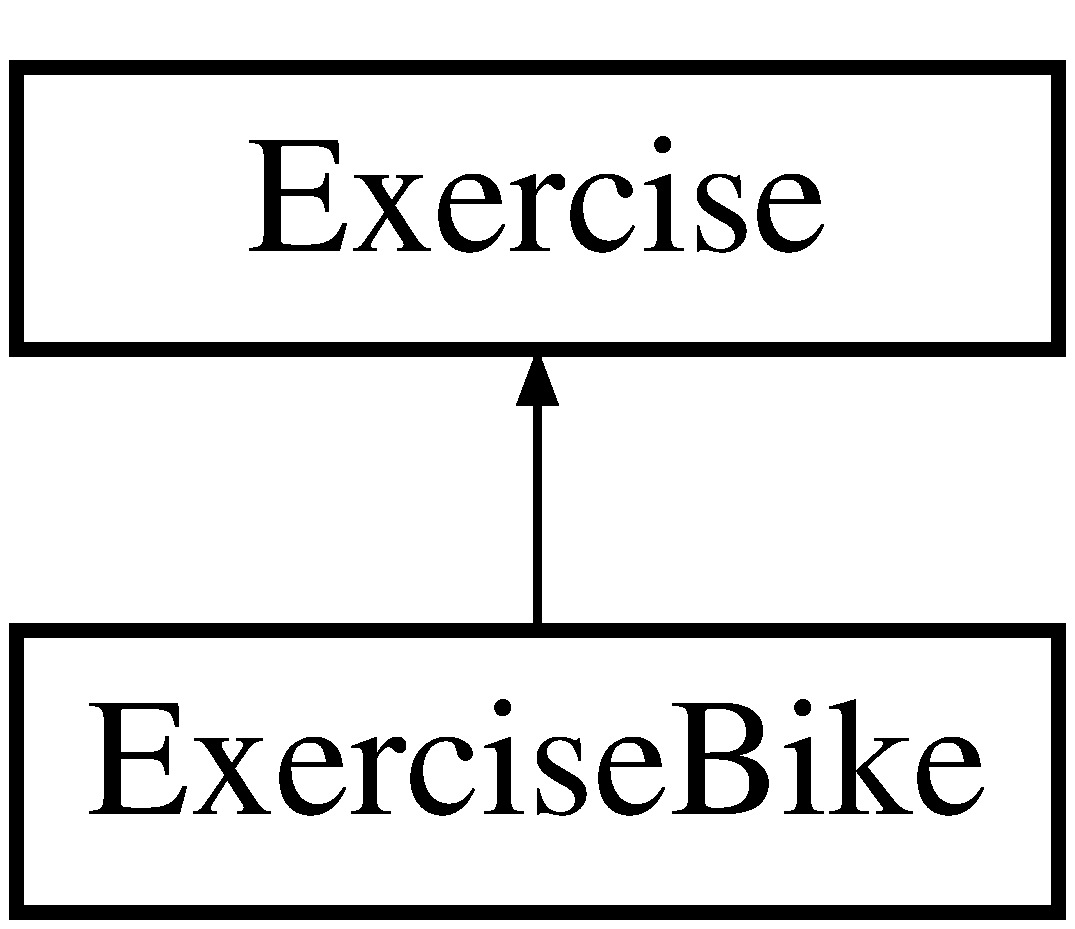
\includegraphics[height=2.000000cm]{class_exercise_bike}
\end{center}
\end{figure}
\subsection*{Public Member Functions}
\begin{DoxyCompactItemize}
\item 
\hyperlink{class_exercise}{Exercise} $\ast$ \hyperlink{class_exercise_bike_a399ba0e490a455147245e79ca814be24}{clone} ()
\item 
\hypertarget{class_exercise_bike_a3cac91aa3fb57c12b3e1e87d527a3291}{}void {\bfseries work\+\_\+out} ()\label{class_exercise_bike_a3cac91aa3fb57c12b3e1e87d527a3291}

\end{DoxyCompactItemize}


\subsection{Member Function Documentation}
\hypertarget{class_exercise_bike_a399ba0e490a455147245e79ca814be24}{}\index{Exercise\+Bike@{Exercise\+Bike}!clone@{clone}}
\index{clone@{clone}!Exercise\+Bike@{Exercise\+Bike}}
\subsubsection[{clone()}]{\setlength{\rightskip}{0pt plus 5cm}{\bf Exercise}$\ast$ Exercise\+Bike\+::clone (
\begin{DoxyParamCaption}
{}
\end{DoxyParamCaption}
)\hspace{0.3cm}{\ttfamily [inline]}, {\ttfamily [virtual]}}\label{class_exercise_bike_a399ba0e490a455147245e79ca814be24}
string Exercise\+Name; 

Implements \hyperlink{class_exercise_ae8dd16c306375ec553ab046e26bea59a}{Exercise}.



The documentation for this class was generated from the following file\+:\begin{DoxyCompactItemize}
\item 
Gym\+Pesicka\+V00807592/\+Gym\+Pesicka\+V00807592/Gym\+Pesicka\+V00807592.\+cpp\end{DoxyCompactItemize}

\hypertarget{class_factory}{}\section{Factory Class Reference}
\label{class_factory}\index{Factory@{Factory}}
\subsection*{Static Public Member Functions}
\begin{DoxyCompactItemize}
\item 
\hypertarget{class_factory_a68c8c516bcfdd5639b08e84967d856ea}{}static \hyperlink{class_exercise}{Exercise} $\ast$ {\bfseries choose\+\_\+exercise} (int choice)\label{class_factory_a68c8c516bcfdd5639b08e84967d856ea}

\end{DoxyCompactItemize}


The documentation for this class was generated from the following file\+:\begin{DoxyCompactItemize}
\item 
Gym\+Pesicka\+V00807592/\+Gym\+Pesicka\+V00807592/Gym\+Pesicka\+V00807592.\+cpp\end{DoxyCompactItemize}

\hypertarget{classthe_elliptical}{}\section{the\+Elliptical Class Reference}
\label{classthe_elliptical}\index{the\+Elliptical@{the\+Elliptical}}
Inheritance diagram for the\+Elliptical\+:\begin{figure}[H]
\begin{center}
\leavevmode
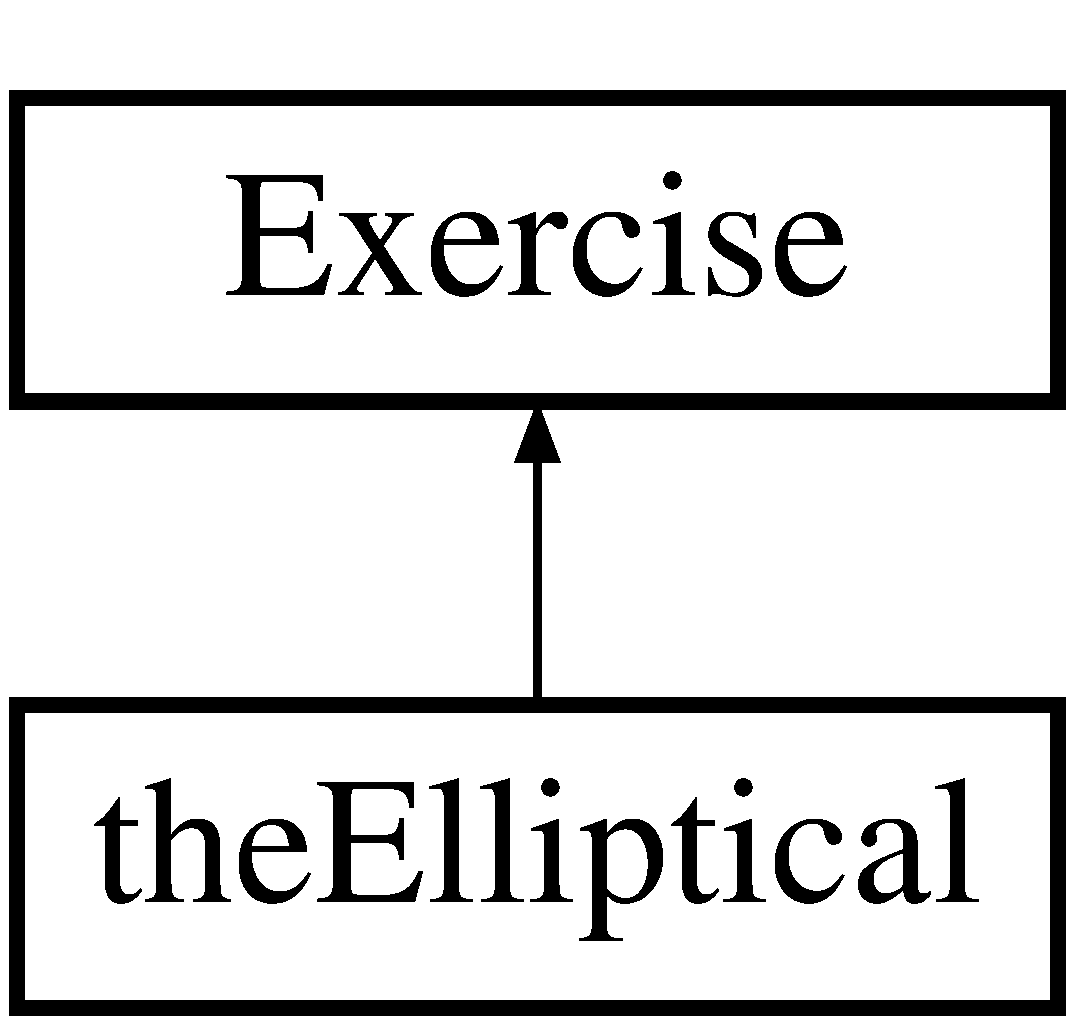
\includegraphics[height=2.000000cm]{classthe_elliptical}
\end{center}
\end{figure}
\subsection*{Public Member Functions}
\begin{DoxyCompactItemize}
\item 
\hyperlink{class_exercise}{Exercise} $\ast$ \hyperlink{classthe_elliptical_a650c1be9061ad3c25eda5017d50f91be}{clone} ()
\item 
\hypertarget{classthe_elliptical_a0a5f2bc9bbae030464f1cf6af282dedd}{}void {\bfseries work\+\_\+out} ()\label{classthe_elliptical_a0a5f2bc9bbae030464f1cf6af282dedd}

\end{DoxyCompactItemize}


\subsection{Member Function Documentation}
\hypertarget{classthe_elliptical_a650c1be9061ad3c25eda5017d50f91be}{}\index{the\+Elliptical@{the\+Elliptical}!clone@{clone}}
\index{clone@{clone}!the\+Elliptical@{the\+Elliptical}}
\subsubsection[{clone()}]{\setlength{\rightskip}{0pt plus 5cm}{\bf Exercise}$\ast$ the\+Elliptical\+::clone (
\begin{DoxyParamCaption}
{}
\end{DoxyParamCaption}
)\hspace{0.3cm}{\ttfamily [inline]}, {\ttfamily [virtual]}}\label{classthe_elliptical_a650c1be9061ad3c25eda5017d50f91be}
string Exercise\+Name; 

Implements \hyperlink{class_exercise_ae8dd16c306375ec553ab046e26bea59a}{Exercise}.



The documentation for this class was generated from the following file\+:\begin{DoxyCompactItemize}
\item 
Gym\+Pesicka\+V00807592/\+Gym\+Pesicka\+V00807592/Gym\+Pesicka\+V00807592.\+cpp\end{DoxyCompactItemize}

\hypertarget{classthe_treadmill}{}\section{the\+Treadmill Class Reference}
\label{classthe_treadmill}\index{the\+Treadmill@{the\+Treadmill}}
Inheritance diagram for the\+Treadmill\+:\begin{figure}[H]
\begin{center}
\leavevmode
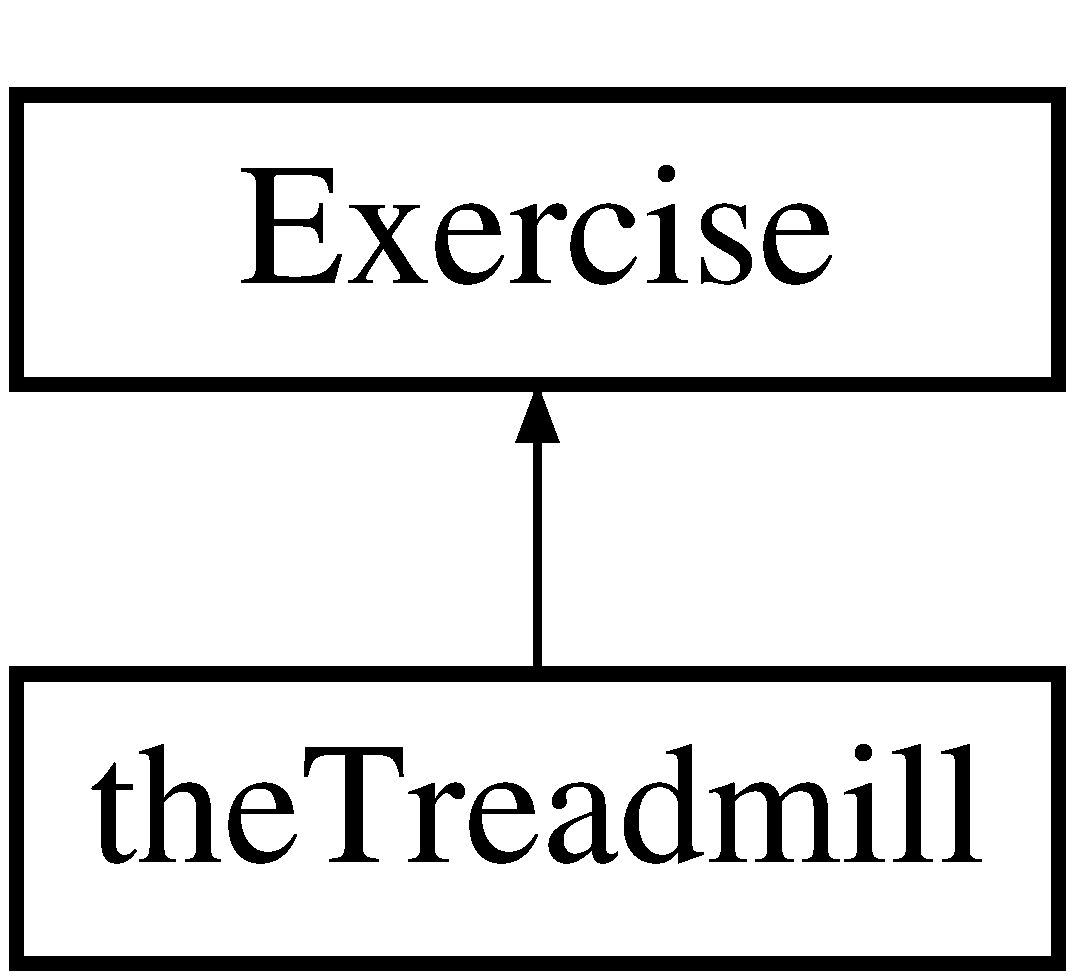
\includegraphics[height=2.000000cm]{classthe_treadmill}
\end{center}
\end{figure}
\subsection*{Public Member Functions}
\begin{DoxyCompactItemize}
\item 
\hyperlink{class_exercise}{Exercise} $\ast$ \hyperlink{classthe_treadmill_af116aacb6c62a04edd1029a6049c1461}{clone} ()
\item 
\hypertarget{classthe_treadmill_a81c9be4911c076ad84651b199e11267e}{}void {\bfseries work\+\_\+out} ()\label{classthe_treadmill_a81c9be4911c076ad84651b199e11267e}

\end{DoxyCompactItemize}


\subsection{Member Function Documentation}
\hypertarget{classthe_treadmill_af116aacb6c62a04edd1029a6049c1461}{}\index{the\+Treadmill@{the\+Treadmill}!clone@{clone}}
\index{clone@{clone}!the\+Treadmill@{the\+Treadmill}}
\subsubsection[{clone()}]{\setlength{\rightskip}{0pt plus 5cm}{\bf Exercise}$\ast$ the\+Treadmill\+::clone (
\begin{DoxyParamCaption}
{}
\end{DoxyParamCaption}
)\hspace{0.3cm}{\ttfamily [inline]}, {\ttfamily [virtual]}}\label{classthe_treadmill_af116aacb6c62a04edd1029a6049c1461}
string Exercise\+Name; 

Implements \hyperlink{class_exercise_ae8dd16c306375ec553ab046e26bea59a}{Exercise}.



The documentation for this class was generated from the following file\+:\begin{DoxyCompactItemize}
\item 
Gym\+Pesicka\+V00807592/\+Gym\+Pesicka\+V00807592/Gym\+Pesicka\+V00807592.\+cpp\end{DoxyCompactItemize}

\hypertarget{class_weight_room}{}\section{Weight\+Room Class Reference}
\label{class_weight_room}\index{Weight\+Room@{Weight\+Room}}
Inheritance diagram for Weight\+Room\+:\begin{figure}[H]
\begin{center}
\leavevmode
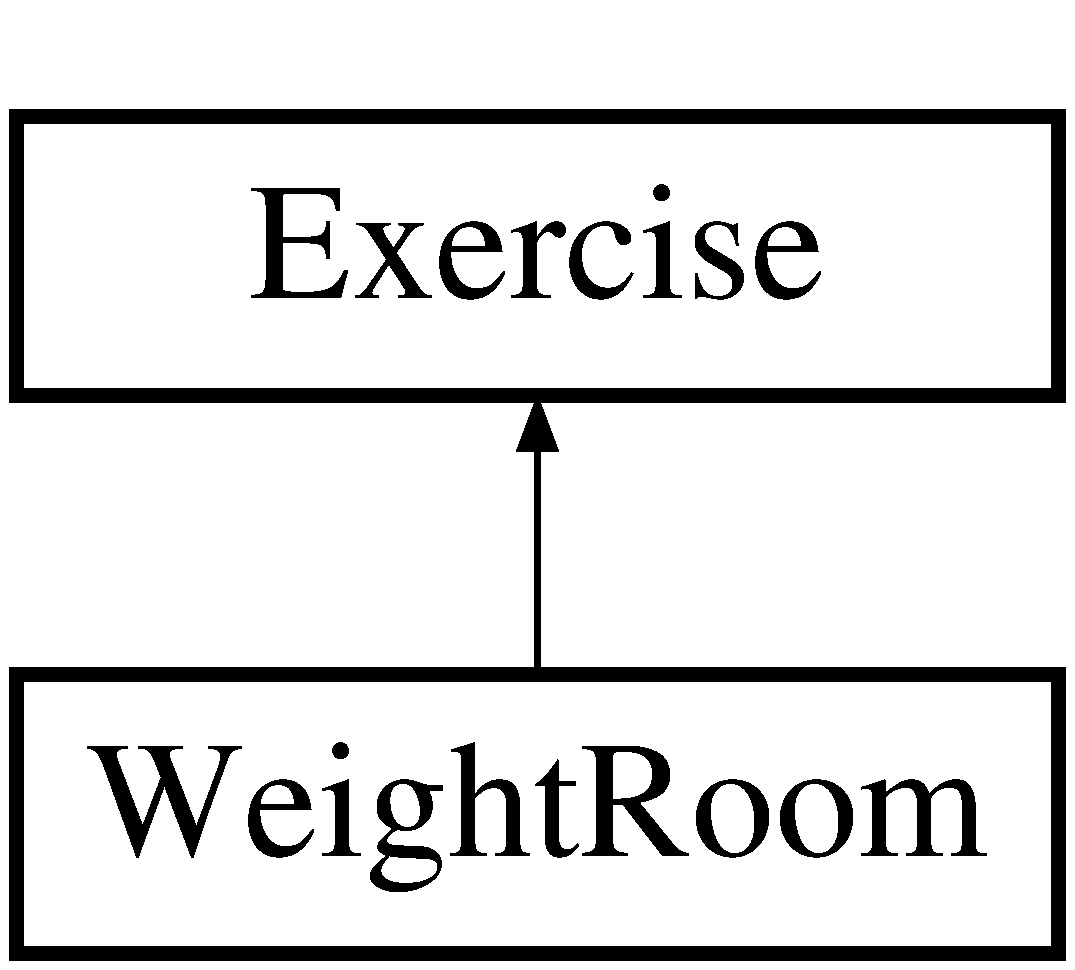
\includegraphics[height=2.000000cm]{class_weight_room}
\end{center}
\end{figure}
\subsection*{Public Member Functions}
\begin{DoxyCompactItemize}
\item 
\hyperlink{class_exercise}{Exercise} $\ast$ \hyperlink{class_weight_room_adc9336a7d4d0f826d8e17e3ac2a0b936}{clone} ()
\item 
\hypertarget{class_weight_room_a20c9e8b1c16e20bf62430fc389af4d3c}{}void {\bfseries work\+\_\+out} ()\label{class_weight_room_a20c9e8b1c16e20bf62430fc389af4d3c}

\end{DoxyCompactItemize}


\subsection{Member Function Documentation}
\hypertarget{class_weight_room_adc9336a7d4d0f826d8e17e3ac2a0b936}{}\index{Weight\+Room@{Weight\+Room}!clone@{clone}}
\index{clone@{clone}!Weight\+Room@{Weight\+Room}}
\subsubsection[{clone()}]{\setlength{\rightskip}{0pt plus 5cm}{\bf Exercise}$\ast$ Weight\+Room\+::clone (
\begin{DoxyParamCaption}
{}
\end{DoxyParamCaption}
)\hspace{0.3cm}{\ttfamily [inline]}, {\ttfamily [virtual]}}\label{class_weight_room_adc9336a7d4d0f826d8e17e3ac2a0b936}
string Exercise\+Name; 

Implements \hyperlink{class_exercise_ae8dd16c306375ec553ab046e26bea59a}{Exercise}.



The documentation for this class was generated from the following file\+:\begin{DoxyCompactItemize}
\item 
Gym\+Pesicka\+V00807592/\+Gym\+Pesicka\+V00807592/Gym\+Pesicka\+V00807592.\+cpp\end{DoxyCompactItemize}

%--- End generated contents ---

% Index
\backmatter
\newpage
\phantomsection
\clearemptydoublepage
\addcontentsline{toc}{chapter}{Index}
\printindex

\end{document}
